\section{Results}

\subsection{Main Finding: Hypothesis Refuted}

The CV-based detection mechanism achieves \textbf{AUC = 0.0}, decisively failing the $\geq$0.75 gate.

\subsection{CV Distribution}

\begin{table}[h]
\centering
\begin{tabular}{@{}lll@{}}
\toprule
Feature Type & CV Value & Expected \\
\midrule
Background (spurious) & 0.0393 & Low ($<$ 0.15) \\
Bird Type (core) & 0.0360 & High ($>$ 0.20) \\
\textbf{Difference} & 0.0033 & --- \\
\bottomrule
\end{tabular}
\end{table}

Both feature types show nearly identical CV values ($\sim$0.04). The hypothesized separation does not manifest.

\begin{figure}[h]
\centering
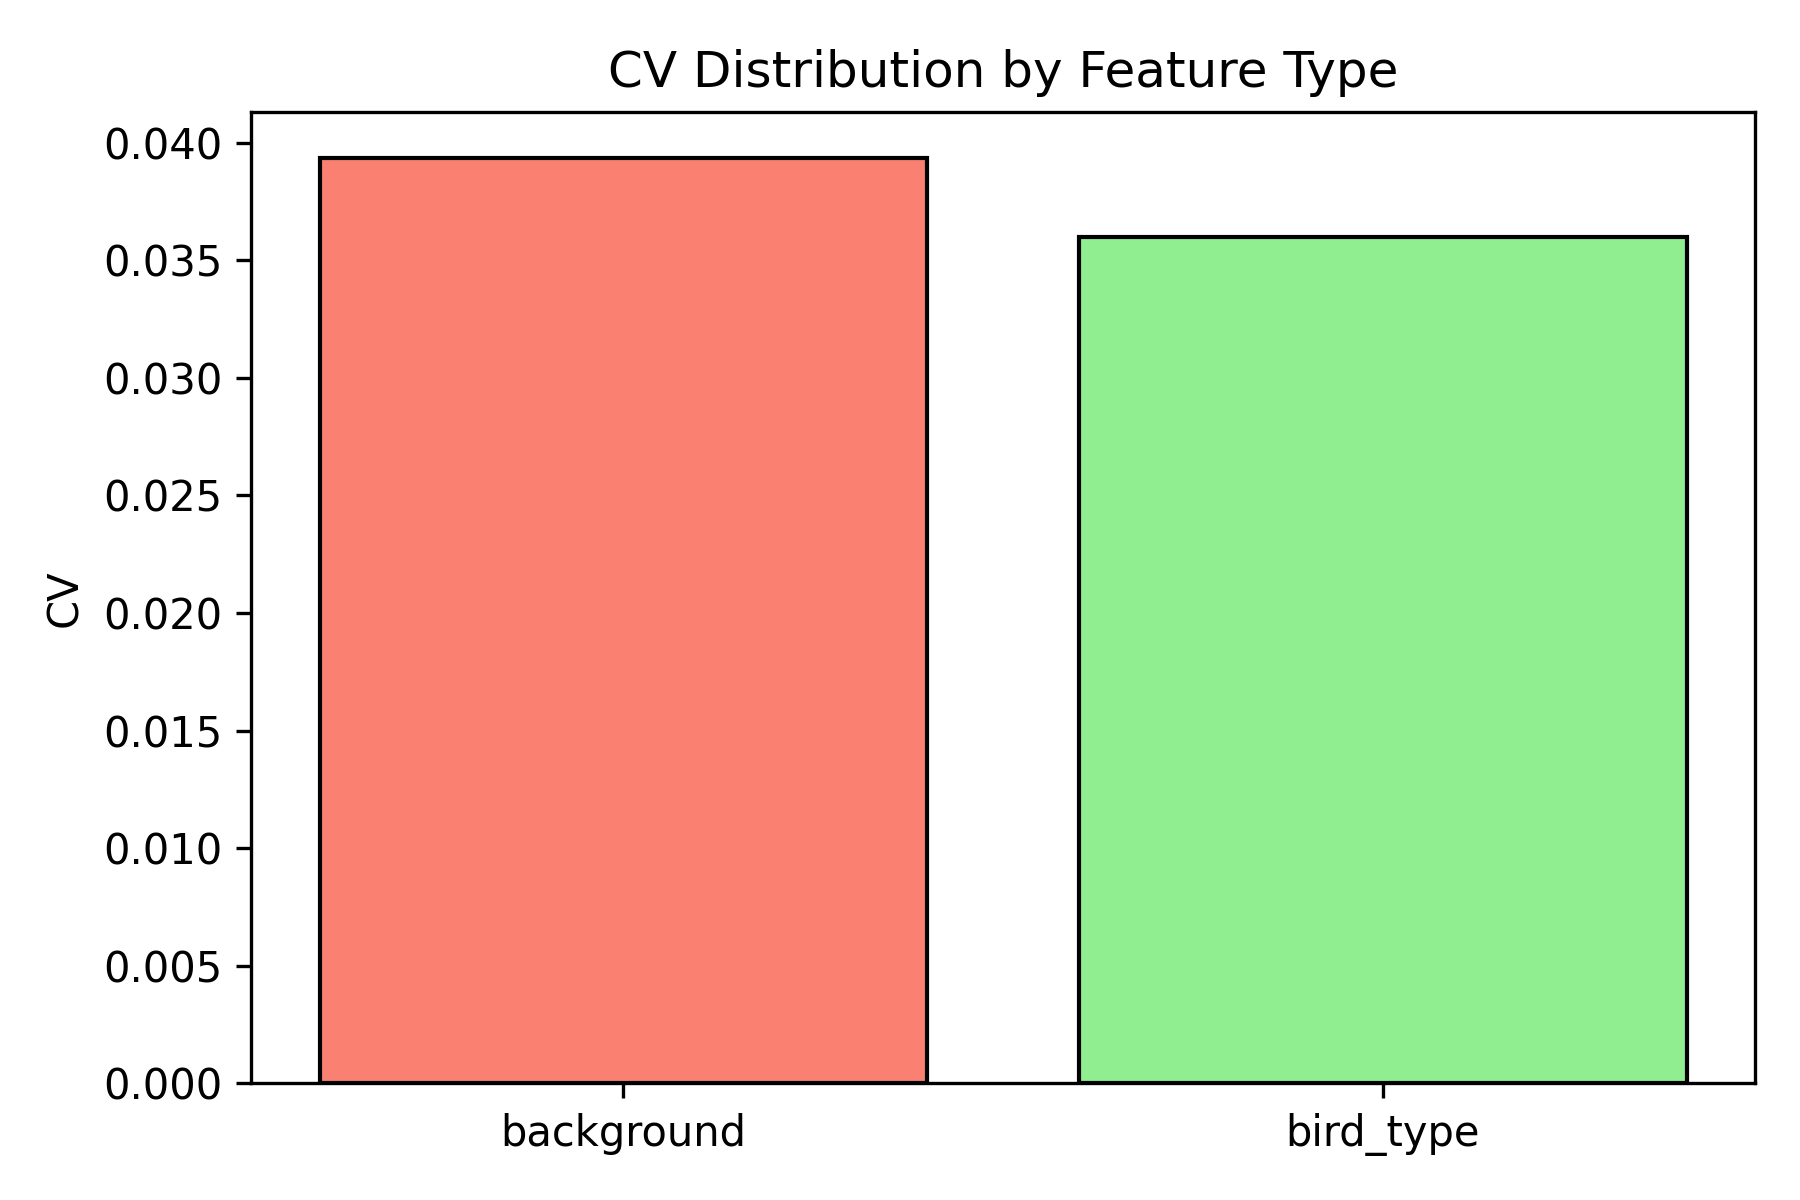
\includegraphics[width=0.8\columnwidth]{figures/cv_distribution.png}
\caption{CV distribution shows both features cluster in the same region with no separation.}
\label{fig:cv_distribution}
\end{figure}

\subsection{Direction Reversal}

The hypothesis predicted: CV(spurious) $<$ CV(core)

Observed: CV(spurious) = 0.0393 $>$ CV(core) = 0.0360

The direction is marginally reversed, though within noise. With only 2 feature types, this reversal yields AUC = 0.0.

\subsection{Probe Trajectory Analysis}

\begin{table}[h]
\centering
\begin{tabular}{@{}ll@{}}
\toprule
Feature Type & Trajectory Pattern \\
\midrule
Background & Flat at $\sim$100\% across all C \\
Bird Type & Flat at $\sim$100\% across all C \\
\bottomrule
\end{tabular}
\end{table}

\begin{figure}[h]
\centering
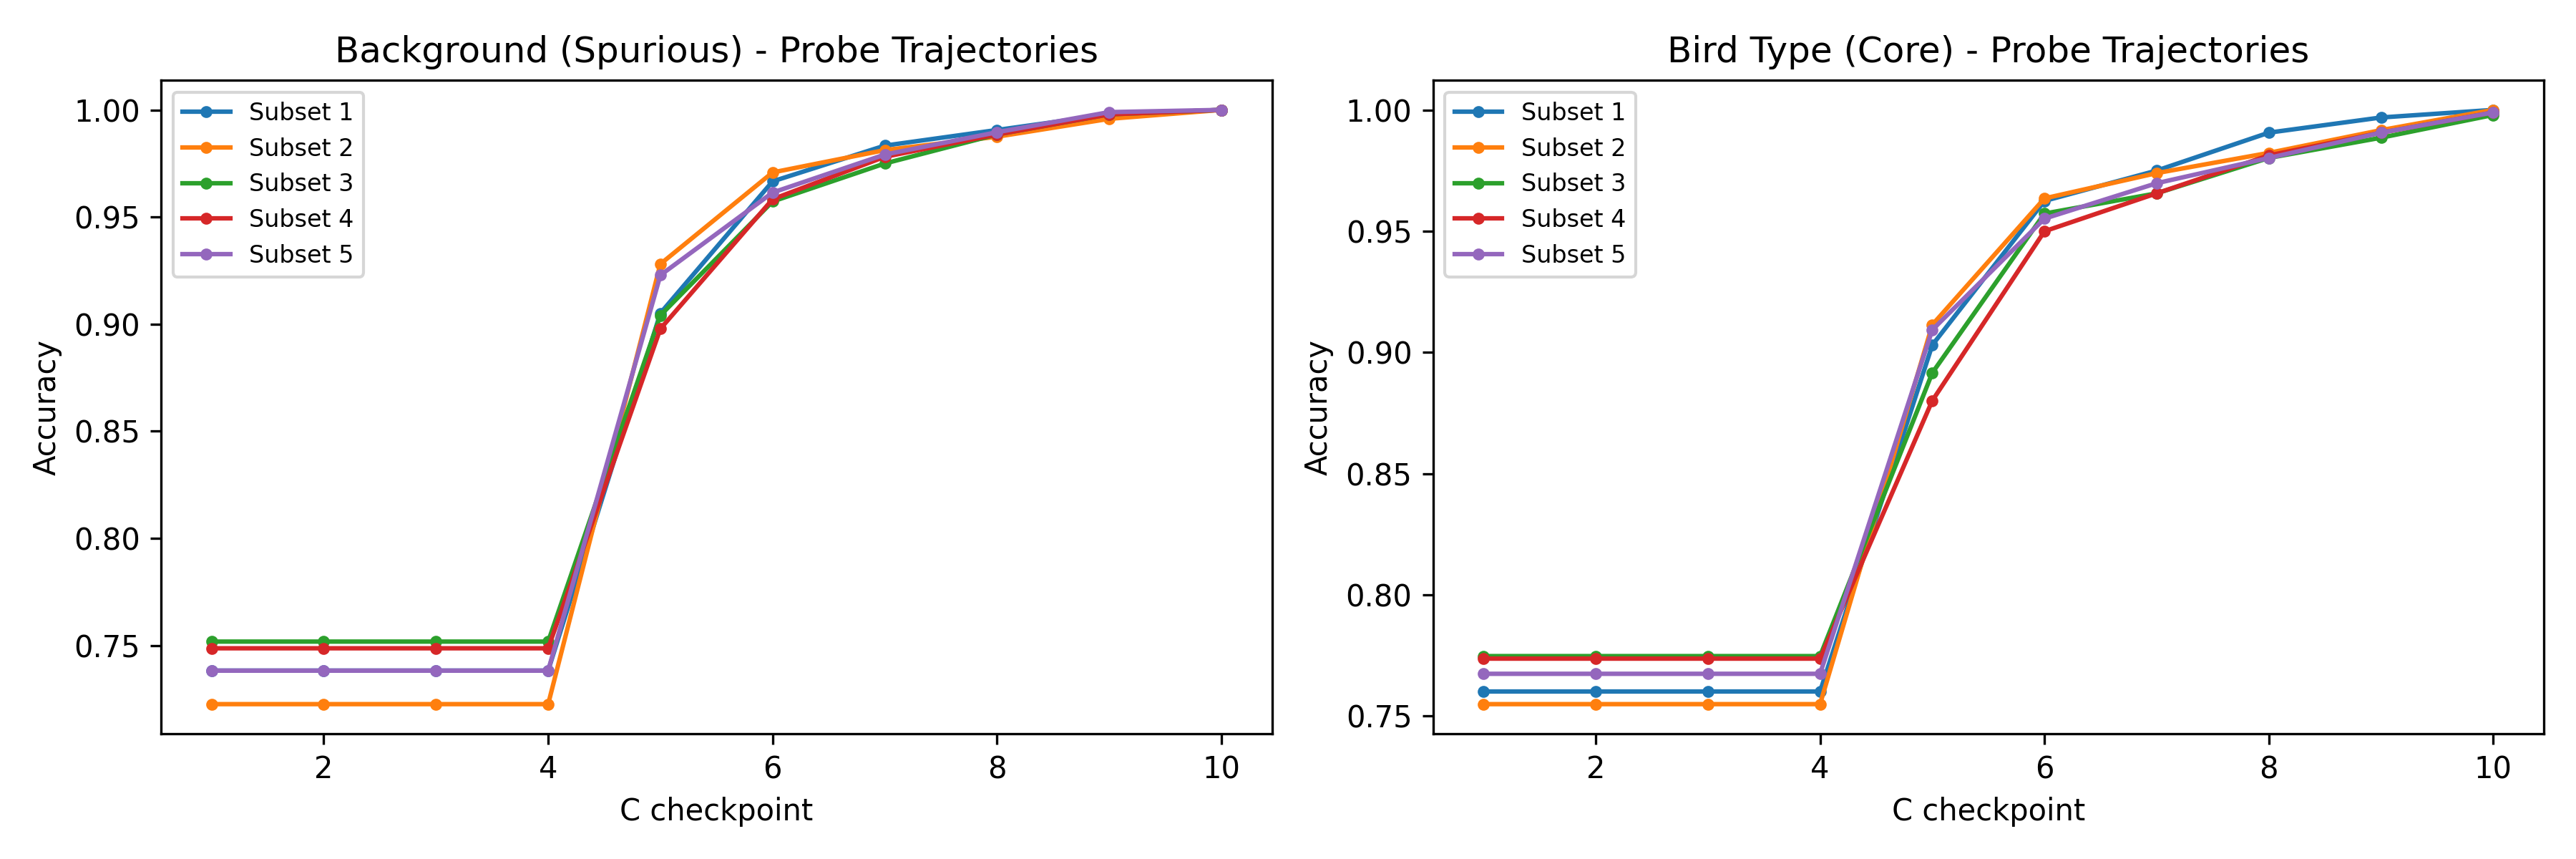
\includegraphics[width=0.8\columnwidth]{figures/trajectories.png}
\caption{Probe accuracy trajectories are flat --- features are already learned.}
\label{fig:trajectories}
\end{figure}

\subsection{Gate Evaluation}

\begin{table}[h]
\centering
\begin{tabular}{@{}llll@{}}
\toprule
Metric & Value & Threshold & Status \\
\midrule
AUC & 0.0 & $\geq$ 0.75 & \textbf{FAIL} \\
\bottomrule
\end{tabular}
\end{table}

\begin{figure}[h]
\centering
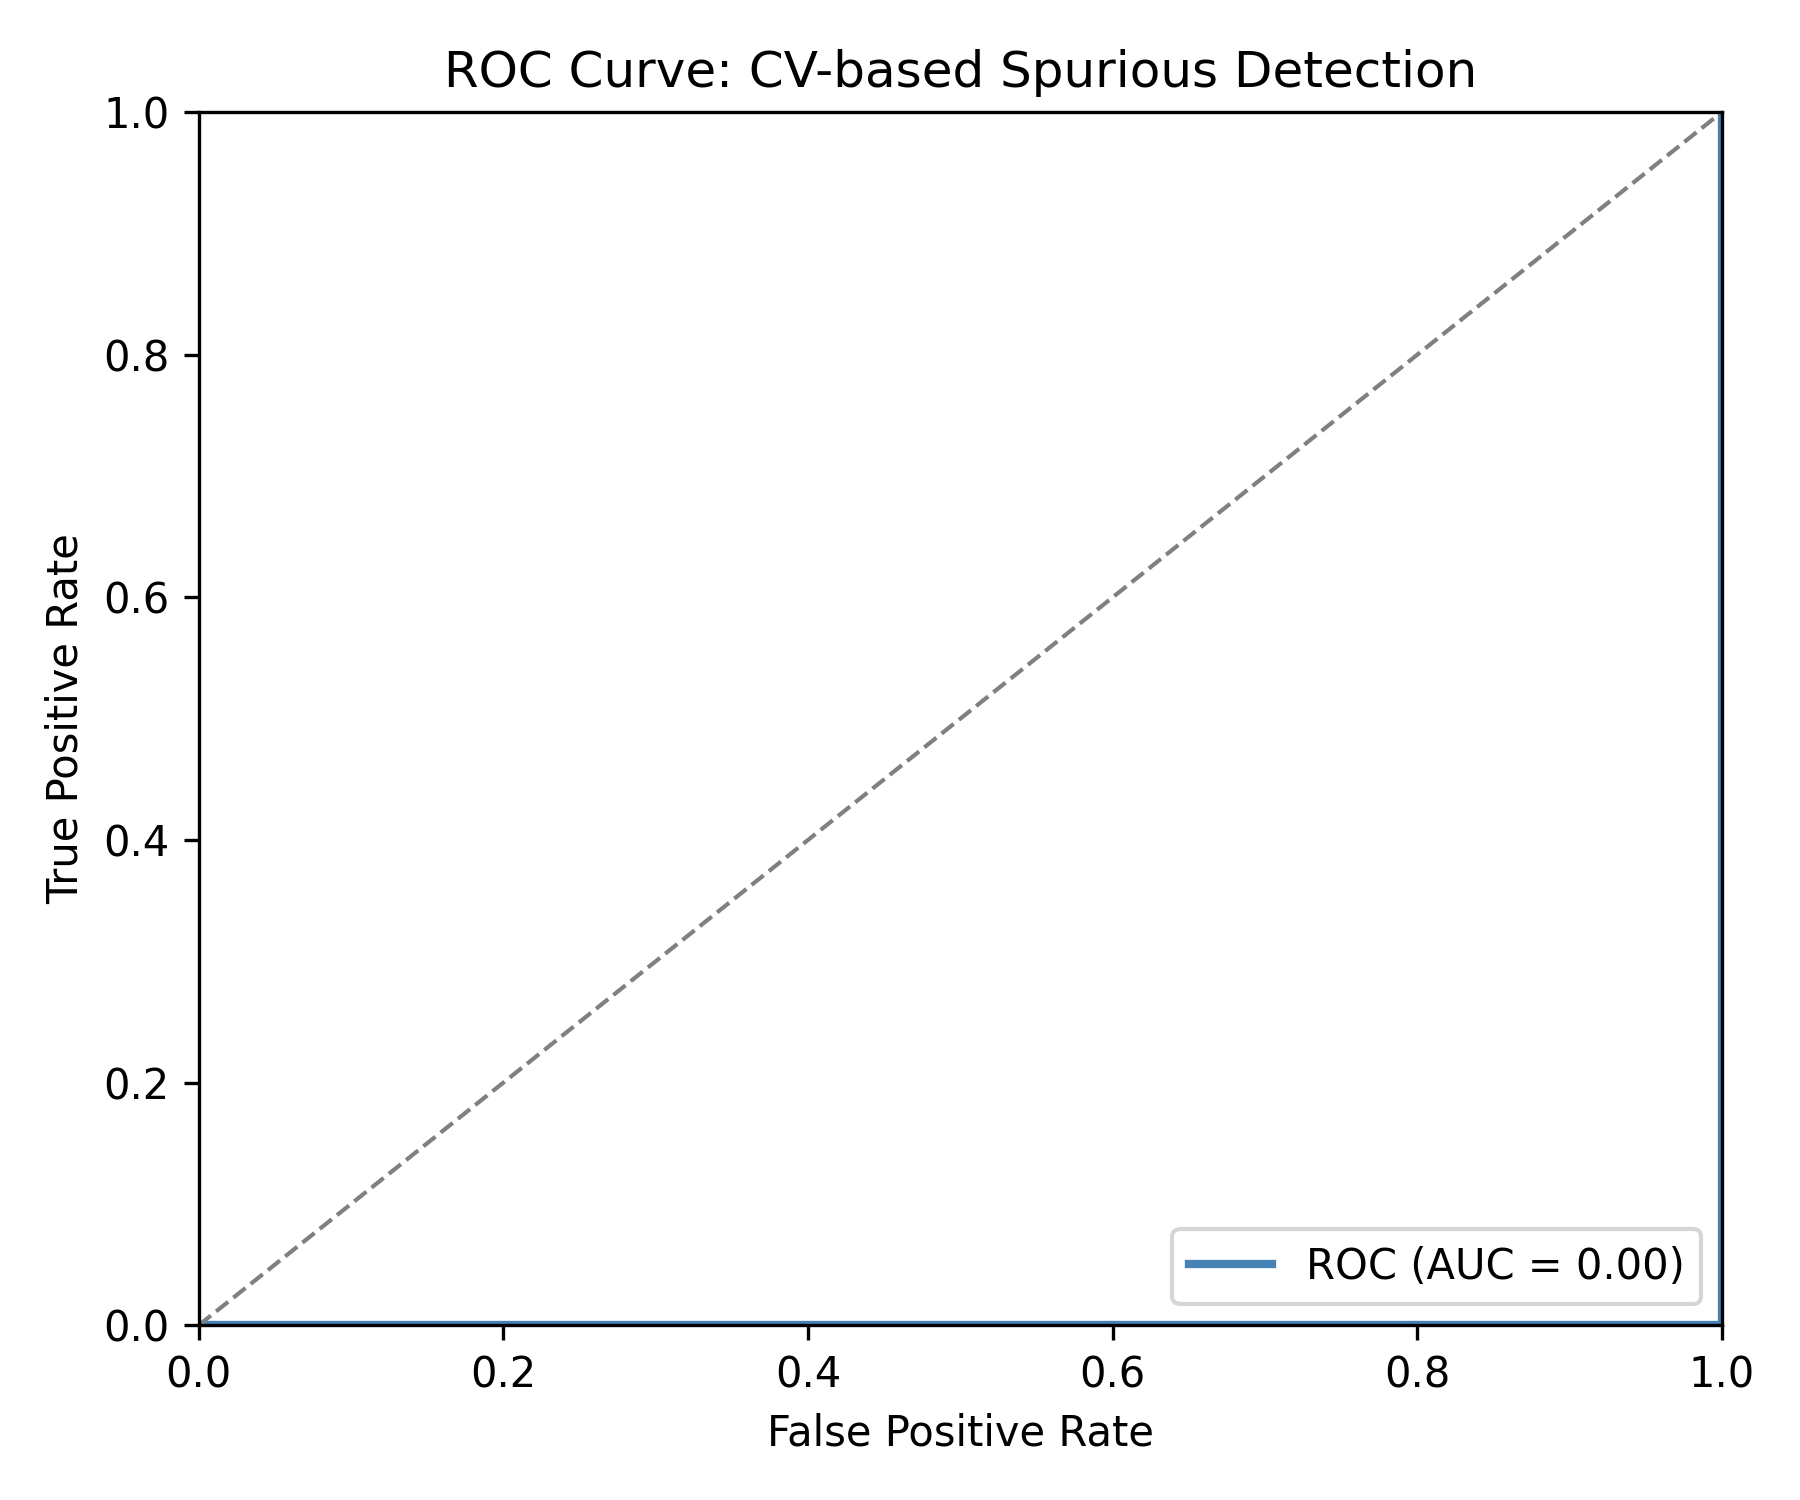
\includegraphics[width=0.8\columnwidth]{figures/roc_curve.png}
\caption{ROC curve hugs the diagonal, indicating no discriminative power.}
\label{fig:roc_curve}
\end{figure}
